% =====================================================================
% Avaliação da Qualidade de Produto de Software: DF no Ponto
% Entrega 1 (Fases 1 e 2) - Modelo SBC
% Compilar com pdfLaTeX (padrão do Overleaf)
% Requer: sbc-template.sty (versão corrigida) na mesma pasta do projeto
% =====================================================================
\documentclass[11pt,a4paper]{article}

\usepackage{sbc-template}   % modelo SBC (arquivo sbc-template.sty corrigido)
\usepackage{graphicx,url}
\usepackage[brazil]{babel}
\usepackage[utf8]{inputenc}
\usepackage{booktabs}
\usepackage{tabularx}
\usepackage{amsmath} % Adicionado para suportar fórmulas matemáticas nas métricas
\usepackage{tikz}
\usepackage{float}
\usetikzlibrary{positioning}
\usepackage{hyperref}
\hypersetup{colorlinks=true,urlcolor=blue,linkcolor=black,citecolor=black,
            pdftitle={Avaliação da Qualidade de Produto de Software: DF no Ponto}}

\title{\textbf{Avaliação da Qualidade de Produto de Software:\\ DF no Ponto}\\
       \vspace{0.5em}
       {\large \textbf{Relatório da Entrega 1 --- Fases 1 e 2 do Processo de Avaliação}}}

\author{Cristiano Borges de Morais \\ João Guilherme Capozzi Gonçalves \\
        João Guilherme Lima Veras Fonseca \\ Pedro Ramos Sousa Reis \\
        Rodrigo Braz Ferreira Gontijo \\ Vitor Pereira Bessa}

\address{Universidade de Brasília (UnB) --- Faculdade de Ciências e Tecnologias\\
         em Engenharia (FCTE), Brasília -- DF -- Brasil}

\begin{document}

\maketitle

\begin{resumo}
Este relatório apresenta a primeira entrega do projeto final da disciplina Qualidade de Software 1, que avalia a qualidade do aplicativo móvel DF no Ponto, ferramenta oficial do transporte público do Distrito Federal. O relatório cobre as duas primeiras fases do processo recomendado pela ISO/IEC 25040: requisitos da avaliação (Fase 1) e especificação da avaliação (Fase 2). Utilizou-se a abordagem Goal-Question-Metric (GQM) para desdobrar os objetivos de Adequação Funcional, Confiabilidade e Portabilidade em métricas quantitativas e critérios de julgamento. São fornecidos os links do repositório, portal de documentação e tabela de contribuição.
\end{resumo}

\vspace{0.5em}
\noindent \textbf{Palavras-chave:} Qualidade de Software, ISO/IEC 25010, GQM, Mobilidade Urbana, DF no Ponto.

% ---------------------------------------------------------------------
\section{Introdução}
\label{sec:intro}

O transporte público desempenha um papel fundamental na mobilidade urbana do Distrito Federal. Nesse contexto, o aplicativo DF no Ponto tornou-se a ferramenta oficial e amplamente utilizada por milhares de cidadãos diariamente para planejar rotas, verificar horários e acompanhar as linhas de ônibus em tempo real. No entanto, passageiros frequentemente relatam problemas graves na experiência de uso: ônibus que ``somem'' do mapa interativo, previsões de horários que não coincidem com a realidade e fechamentos abruptos (\textit{crashes}) do sistema exatamente no momento de decisão de embarque. Estudos sobre avaliações de usuários de aplicativos móveis confirmam que falhas de estabilidade e precisão funcional figuram entre as principais causas de rejeição e desinstalação~\cite{khalid2015,minelli2015}. Tais falhas geram atrasos sistemáticos, perda de tempo e insatisfação generalizada, minando a confiança da população no serviço digital.

O objetivo geral deste trabalho é realizar uma avaliação rigorosa da qualidade de software do produto DF no Ponto, sob a perspectiva do usuário final, com foco em identificar fragilidades e propor melhorias técnicas concretas. Para conduzir essa análise de forma estruturada e metodologicamente fundamentada, este trabalho utiliza o modelo de qualidade da norma ISO/IEC 25010, que fornece características padronizadas para a avaliação de sistemas~\cite{deissenboeck2009}, aliado à abordagem Goal-Question-Metric (GQM)~\cite{basili1988}. O GQM permite derivar de forma sistemática métricas operacionais e quantitativas a partir dos objetivos conceituais de medição, garantindo que os dados coletados estejam diretamente atrelados à percepção de valor do passageiro.

O restante deste artigo está organizado da seguinte forma: a Seção~\ref{sec:referencial} apresenta o referencial teórico; a Seção~\ref{sec:metodologia} descreve a metodologia de avaliação; a Seção~\ref{sec:fase1} detalha a Fase~1 (requisitos da avaliação); a Seção~\ref{sec:fase2} especifica a Fase~2 (desdobramento GQM); e o Apêndice~\ref{ap:contribuicao} contém a tabela de contribuição.

% ---------------------------------------------------------------------
\section{Referencial Teórico}
\label{sec:referencial}

Nesta seção, contextualizam-se os conceitos fundamentais que sustentam a avaliação de qualidade conduzida neste projeto, abordando os padrões internacionais de qualidade de produto de software, os processos padronizados de avaliação, a abordagem metodológica de medição e as evidências empíricas sobre a qualidade em aplicações móveis.

A base normativa deste trabalho apoia-se na família de normas ISO/IEC 25000 (SQuaRE --- \textit{Systems and software Quality Requirements and Evaluation})~\cite{iso25000}, que estabelece diretrizes e modelos de referência para orientar a especificação e a avaliação da qualidade de produtos de software. Em especial, a norma ISO/IEC 25010~\cite{iso25010} define o modelo de qualidade de produto organizado hierarquicamente em características e subcaracterísticas, tais como Adequação Funcional, Confiabilidade e Portabilidade, provendo vocabulário comum e critérios unificados de análise. Conforme discutido por Deissenboeck et al.~\cite{deissenboeck2009}, modelos de qualidade genéricos devem ser selecionados e adaptados aos propósitos e ao contexto específico de uso de cada sistema, o que fundamenta a escolha criteriosa das características priorizadas nesta pesquisa.

Para operacionalizar a condução da análise, adota-se o processo estabelecido pela norma ISO/IEC 25040~\cite{iso25040}, a qual prescreve quatro fases sequenciais: o estabelecimento dos requisitos da avaliação (Fase~1), a especificação da avaliação (Fase~2), o planejamento (Fase~3) e a execução para obtenção dos resultados e julgamento (Fase~4). O escopo do presente relatório compreende integralmente as Fases~1 e~2, delimitando o escopo a partir da perspectiva do usuário e traduzindo os requisitos em especificações formais de medição.

A definição e o alinhamento das métricas foram estruturados sob a abordagem \textit{Goal-Question-Metric} (GQM), concebida por Basili e Rombach~\cite{basili1988} e formalizada em Basili et al.~\cite{basili1994}. O método estabelece um fluxo hierárquico descendente em que objetivos conceituais de medição (\textit{Goals}) são formulados para caracterizar o propósito do projeto; tais metas são subsequentemente desdobradas em questões avaliativas operacionais (\textit{Questions}), as quais determinam objetivamente as métricas quantitativas (\textit{Metrics}) a serem coletadas. Essa metodologia assegura que cada dado gerado na avaliação possua justificativa técnica e rastreabilidade direta com os anseios das partes interessadas.

Por fim, a fundamentação empírica específica sobre sistemas móveis apoia-se em estudos da literatura especializada. Khalid et al.~\cite{khalid2015}, ao analisarem mais de 20 mil avaliações de usuários em lojas de aplicativos, identificaram que interrupções forçadas (\textit{crashes}), divergências em dados funcionais e falhas no tratamento de conexões instáveis constituem as causas preponderantes de insatisfação e abandono de software móvel. De modo análogo, Minelli et al.~\cite{minelli2015} ressaltam a centralidade da maturidade e da estabilidade no uso diário de aplicações. Tais constatações empíricas convergem diretamente com os problemas relatados pelos passageiros do Distrito Federal e justificam tecnicamente o direcionamento da avaliação para Adequação Funcional, Confiabilidade e Portabilidade.

% ---------------------------------------------------------------------
\section{Metodologia de Desenvolvimento do Projeto}
\label{sec:metodologia}

A metodologia de avaliação adotada neste trabalho fundamenta-se no processo estabelecido pela norma ISO/IEC 25010, adaptado para a análise externa do aplicativo móvel \textit{DF no Ponto}. O processo executado nesta primeira entrega divide-se em duas fases fundamentais. Na Fase 1 (Requisitos da Avaliação), o escopo foi delimitado com base na perspectiva do usuário final (passageiro), priorizando as características de Adequação Funcional, Confiabilidade e Portabilidade a partir do modelo de qualidade da ISO/IEC 25010~\cite{iso25010}.

Na Fase 2 (Especificação da Avaliação), a modelagem foi operacionalizada através da abordagem \textit{Goal-Question-Metric} (GQM)~\cite{basili1994,basili1988}. Essa estrutura garantiu que os objetivos conceituais de qualidade fossem desdobrados em questões avaliativas precisas e, consequentemente, em métricas quantitativas com critérios de julgamento rigorosos, assegurando a rastreabilidade técnica dos testes que serão executados. A adoção de testes de caixa preta está em consonância com abordagens consolidadas na literatura para avaliação externa de produtos de software~\cite{deissenboeck2009}.

Toda a documentação dinâmica (\textit{GitPage}), artefatos de avaliação e este relatório gerado em \LaTeX\ (modelo SBC) estão mantidos sob controle de versão e acessíveis em:

\begin{itemize}
    \item \textbf{Repositório GitHub:} \\
    {\small \url{https://github.com/FCTE-Qualidade-de-Software-1/2026-2_T02_CAROL_SHAW}}
    \item \textbf{GitPage:} \\
    {\small \url{https://fcte-qualidade-de-software-1.github.io/2026-2_T02_CAROL_SHAW/}}
\end{itemize}

% ---------------------------------------------------------------------
\section{Fase 1: Requisitos da Avaliação}
\label{sec:fase1}

\subsection{Propósito, Destinatários e Uso dos Resultados}
O propósito desta avaliação é analisar o aplicativo DF no Ponto sob a perspectiva do usuário final, a fim de identificar oportunidades de melhoria técnica. Os destinatários são: (i)~Semob-DF e operadoras parceiras (interessados em melhorias); (ii)~passageiros (beneficiários); e (iii)~avaliadores da disciplina (requisitantes acadêmicos). Os resultados subsidiarão o julgamento da qualidade na Fase 4 e fundamentarão as ações de melhoria exigidas na Entrega 2.

Adicionalmente, o propósito desta avaliação alinha-se aos Objetivos de Desenvolvimento Sustentável (ODS) da Agenda 2030 da Organização das Nações Unidas~\cite{onu2015}. O projeto vincula-se diretamente ao ODS~11 (Cidades e Comunidades Sustentáveis), com foco na Meta~11.2, ao promover o acesso a sistemas de transporte público seguros, sustentáveis e previsíveis por meio de informações precisas de itinerários e paradas. De forma complementar, relaciona-se ao ODS~9 (Indústria, Inovação e Infraestrutura), em sua Meta~9.1, ao incentivar o aprimoramento da infraestrutura digital e a modernização tecnológica dos serviços essenciais de mobilidade urbana no Distrito Federal.

\subsection{Requisitante, Partes Interessadas, Papéis e Necessidades}
\label{sec:stakeholders}

O Quadro~\ref{tab:stakeholders} sintetiza as partes interessadas, reforçando a convergência de necessidades para os focos de qualidade adotados nesta avaliação.

\begin{table}[h]
\centering
\caption{Partes interessadas, papéis e influência na avaliação.}
\label{tab:stakeholders}
\scriptsize
\begin{tabularx}{\textwidth}{>{\raggedright\arraybackslash}p{2.5cm} >{\raggedright\arraybackslash}p{2.5cm} X X}
\toprule
\textbf{Parte interessada} & \textbf{Papel} & \textbf{Necessidade principal} & \textbf{Influência} \\
\midrule
Passageiros (STPC-DF) & Usuários finais & Horários precisos e app estável em qualquer celular & Priorizam correção funcional, maturidade e adaptabilidade \\
Equipe (estudantes) & Executores & Aplicar a norma ISO/IEC 25010 com rigor analítico & Direcionam para testes de caixa preta \\
Avaliadores (disciplina) & Requisitantes & Verificar a correta aplicação do processo de avaliação & Avaliam consistência metodológica \\
Semob-DF & Gestores & Atender a população com eficiência & Destinatários das melhorias \\
\bottomrule
\end{tabularx}
\end{table}

\subsection{Produto, Escopo e Exclusões}
O produto avaliado é o app móvel (Android/iOS) DF no Ponto em produção. O escopo abrange as funcionalidades centrais de pesquisa de rotas e consulta de horários. A avaliação é externa (\textit{caixa preta}), focada na interface e interação de rede. Estão \textbf{fora do escopo}: eficiência técnica de backend, manutenibilidade do código-fonte, usabilidade estética, segurança da base de dados e funcionamento em plataformas web/tablets.

\subsection{Seleção das Características e Justificativa (ISO/IEC 25010)}
Com base na norma e nas dores reportadas pelos usuários, foram priorizadas três características:
\begin{enumerate}
    \item \textbf{Adequação Funcional (P1):} Sem horários e trajetos precisos (correção e completude), o aplicativo perde sua finalidade primária, justificando a prioridade máxima. Estudos de avaliação de aplicativos de mobilidade urbana apontam a precisão funcional como o atributo de maior impacto na satisfação do usuário~\cite{khalid2015}.
    \item \textbf{Confiabilidade (P2):} Passageiros usam o app sob instabilidade de rede. Falhas de maturidade (\textit{crashes}) durante o embarque tornam a ferramenta inutilizável em momentos críticos~\cite{minelli2015}.
    \item \textbf{Portabilidade (P3):} A diversidade demográfica do DF exige adaptabilidade a variados tamanhos de tela e versões de sistemas operacionais~\cite{deissenboeck2009}.
\end{enumerate}

\begin{figure}[h]
\centering
\resizebox{0.85\textwidth}{!}{%
\begin{tikzpicture}
  [raiz/.style={rectangle,rounded corners,draw,fill=blue!12,font=\small\bfseries,
                align=center,text width=4.6cm,minimum height=1.0cm},
   sel/.style={rectangle,draw,fill=green!18,font=\footnotesize\bfseries,
               align=center,text width=3.6cm,minimum height=1.05cm},
   nao/.style={rectangle,draw=black!40,fill=black!4,font=\scriptsize,
               text=black!60,align=center,text width=2.5cm,minimum height=0.85cm}]
\node[raiz] (raiz) at (4.05,2.3) {Qualidade de Produto de Software\\ ISO/IEC 25010};
\node[sel] (af) at (0,0) {Adequação Funcional\\ {\scriptsize prioridade 1}};
\node[sel] (cf) at (4.05,0) {Confiabilidade\\ {\scriptsize prioridade 2}};
\node[sel] (po) at (8.1,0) {Portabilidade\\ {\scriptsize prioridade 3}};
\draw[->,thick] (raiz.south) -- (af.north);
\draw[->,thick] (raiz.south) -- (cf.north);
\draw[->,thick] (raiz.south) -- (po.north);
\node[nao] (e1) at (-1.70,-1.8) {Eficiência};
\node[nao] (c1) at (1.18,-1.8) {Compatibilidade};
\node[nao] (u1) at (4.05,-1.8) {Usabilidade};
\node[nao] (s1) at (6.93,-1.8) {Segurança};
\node[nao] (m1) at (9.80,-1.8) {Manutenibilidade};
\draw[dashed,rounded corners,black!40] (-3.10,-2.45) rectangle (11.15,-1.15);
\node[font=\scriptsize\itshape,text=black!55] at (4.0,-2.95)
      {Demais características do modelo (documentadas como fora do escopo)};
\end{tikzpicture}
}
\caption{Diagrama do modelo adaptado com as priorizações. Fonte: elaboração própria (2026).}
\label{fig:modelo}
\end{figure}

% ---------------------------------------------------------------------
\section{Fase 2: Especificação da Avaliação}
\label{sec:fase2}

A etapa de especificação traduz as subcaracterísticas de Portabilidade, Confiabilidade e Adequação Funcional em métricas concretas e mensuráveis, fundamentando-se nas medidas padronizadas pela norma ISO/IEC 25010. Para estruturar o desdobramento analítico, emprega-se o framework \textit{Goal--Question--Metric} (GQM)~\cite{basili1994,basili1988}, garantindo que o procedimento seja padronizado e passível de replicação por terceiros.

\subsection{Desdobramento GQM: Objetivos de Medição}
\label{sec:gqm_objetivos}

O escopo foi desdobrado em seis objetivos de medição conceituais, aderentes aos templates formais da literatura e voltados para o aplicativo DF no Ponto:

\begin{itemize}
    \item \textbf{G1 --- Portabilidade (Adaptabilidade):} \textbf{Analisar} o aplicativo móvel \textbf{com a finalidade de} compreender o comportamento adaptativo da interface gráfica, \textbf{no que se refere à} Adaptabilidade, \textbf{do ponto de vista de} usuários finais com variados modelos de smartphones, \textbf{no contexto de} testes em múltiplos dispositivos físicos e simuladores.
    
    \item \textbf{G2 --- Portabilidade (Instalabilidade):} \textbf{Analisar} o processo de empacotamento, instalação e remoção \textbf{com a finalidade de} avaliar a eficiência dos arquivos nas lojas oficiais, \textbf{no que se refere à} Instalabilidade, \textbf{do ponto de vista de} usuários finais e suporte técnico, \textbf{no contexto de} ciclos limpos de instalação e desinstalação.
    
    \item \textbf{G3 --- Confiabilidade (Maturidade):} \textbf{Analisar} a estabilidade de execução e a frequência de travamentos \textbf{com a finalidade de} compreender o nível de robustez contra falhas abruptas, \textbf{no que se refere à} Maturidade, \textbf{do ponto de vista de} passageiros em trânsito diário, \textbf{no contexto de} sessões de uso contínuo e navegação ativa.
    
    \item \textbf{G4 --- Confiabilidade (Tolerância a Falhas):} \textbf{Analisar} a resiliência operacional do sistema \textbf{com a finalidade de} avaliar o comportamento diante de interrupções de conectividade, \textbf{no que se refere à} Tolerância a Falhas, \textbf{do ponto de vista de} passageiros sujeitos a áreas de sombra e sinal deficiente, \textbf{no contexto de} simulações controladas de queda de internet e ausência de GPS.
    
    \item \textbf{G5 --- Adequação Funcional (Correção):} \textbf{Analisar} a exatidão das previsões de horários e geolocalização \textbf{com a finalidade de} verificar a precisão dos dados entregues, \textbf{no que se refere à} Correção, \textbf{do ponto de vista de} cidadãos que dependem de pontualidade, \textbf{no contexto de} validação cruzada entre o app e a operação real nas ruas.
    
    \item \textbf{G6 --- Adequação Funcional (Completude):} \textbf{Analisar} a cobertura de rotas, linhas e ferramentas de busca \textbf{com a finalidade de} certificar se o conjunto atende às demandas de mobilidade, \textbf{no que se refere à} Completude, \textbf{do ponto de vista de} cidadãos planejando trajetos, \textbf{no contexto de} execução integral do catálogo de tarefas essenciais mapeadas.
\end{itemize}

\subsection{Questões Operacionais e Hipóteses}
\label{sec:gqm_questoes}

O desdobramento das metas conceituais gerou interrogações analíticas focadas em validar os atributos de qualidade, conforme detalhado na Tabela~\ref{tab:questoes_hipoteses}.

\begin{table}[H]
\centering
\caption{Matriz de Questões e Hipóteses Operacionais.}
\label{tab:questoes_hipoteses}
\scriptsize
\renewcommand{\arraystretch}{1.2}
\begin{tabularx}{\textwidth}{l c X X}
\toprule
\textbf{Objetivo} & \textbf{ID} & \textbf{Questão Operacional} & \textbf{Hipótese Preditiva} \\
\midrule
\textbf{G1} & Q1.1 & A interface gráfica se redimensiona sem sobreposições em telas compactas? & Espera-se que telas abaixo de 5" apresentem sobreposições pontuais no mapa. \\
(Adaptab.) & Q1.2 & O aplicativo executa sem erros críticos de compatibilidade em sistemas legados? & Espera-se pleno funcionamento nas versões testadas do Android. \\
\midrule
\textbf{G2} & Q2.1 & O processo de instalação nas lojas oficiais ocorre sem fricção ou corrompimento? & Espera-se sucesso de 100\% nas instalações limpas oficiais. \\
(Instalab.) & Q2.2 & O aplicativo remove totalmente seus dados temporários após a desinstalação? & Espera-se que o sistema deixe vestígios menores em cache no armazenamento. \\
\midrule
\textbf{G3} & Q3.1 & O aplicativo evita encerramentos forçados (\textit{crashes}) durante sessões ativas? & Espera-se alta estabilidade geral, com falhas em picos de dados. \\
(Maturid.) & Q3.2 & O sistema previne congelamentos prolongados de tela (\textit{ANRs})? & Espera-se ocorrência pontual de travamentos leves ao sincronizar bases. \\
\midrule
\textbf{G4} & Q4.1 & O aplicativo trata de forma adequada quedas momentâneas de conexão? & Espera-se telas de carregamento infinito por carência de modo \textit{offline}. \\
(Tol. Falhas) & Q4.2 & O sistema reage apropriadamente à ausência ou desativação de sinal de GPS? & Espera-se emissão de alertas visuais claros para reativar serviços. \\
\midrule
\textbf{G5} & Q5.1 & As previsões de horários de chegada refletem com precisão a realidade? & Espera-se margem de divergência tolerável de poucos minutos. \\
(Correção) & Q5.2 & A geolocalização dos veículos no mapa coincide com a posição espacial real? & Espera-se exatidão satisfatória, sujeita a limitações de hardware externo. \\
\midrule
\textbf{G6} & Q6.1 & O catálogo de fluxos e tarefas essenciais executa de ponta a ponta sem barreiras? & Espera-se que módulos principais operem sem falhas estruturais. \\
(Completude) & Q6.2 & A base de dados de linhas está plenamente sincronizada com a Semob? & Espera-se cobertura integral e correta das linhas troncais cadastradas. \\
\bottomrule
\end{tabularx}
\end{table}

\subsection{Definição das Métricas: Cálculo, Fonte e Coleta}
\label{sec:metricas}

As métricas quantitativas respondem diretamente às questões operacionais, fundamentadas na ISO/IEC 25023. Com exceção das métricas baseadas em tempo, utilizam-se razões normalizadas entre 0 e 1.

\begin{itemize}
    \item \textbf{M1.1 --- Adaptabilidade de Hardware (Telas)} (Q1.1):
    \begin{itemize}
        \item \textit{Fórmula:} $Ts / Tt$ (Telas executadas sem sobreposição ou distorção / Total de telas testadas).
        \item \textit{Fonte / Coleta:} Telas em emuladores e dispositivos físicos de diferentes dimensões; inspeção visual da interface.
        \item \textit{Interpretação:} Maior é melhor (0 a 1).
    \end{itemize}

    \item \textbf{M1.2 --- Adaptabilidade de SO} (Q1.2):
    \begin{itemize}
        \item \textit{Fórmula:} $Os / Ot$ (Versões de SO em que o app funciona sem erros / Total de versões testadas).
        \item \textit{Fonte / Coleta:} Relatório de testes de compatibilidade; execução de fluxos críticos em diferentes versões suportadas.
        \item \textit{Interpretação:} Maior é melhor (0 a 1).
    \end{itemize}

    \item \textbf{M2.1 --- Sucesso de Instalação} (Q2.1):
    \begin{itemize}
        \item \textit{Fórmula:} $Is / It$ (Instalações concluídas na primeira tentativa / Total de tentativas).
        \item \textit{Fonte / Coleta:} Logs de download/instalação; execução de ciclos controlados de instalação.
        \item \textit{Interpretação:} Maior é melhor (0 a 1).
    \end{itemize}

    \item \textbf{M2.2 --- Resíduo Pós-Desinstalação} (Q2.2):
    \begin{itemize}
        \item \textit{Fórmula:} $1 - (Dr / Dt)$ (1 - Tentativas que deixaram arquivos órfãos / Total de desinstalações).
        \item \textit{Fonte / Coleta:} Gerenciamento de armazenamento interno; inspeção do diretório de dados após remoção limpa.
        \item \textit{Interpretação:} Maior é melhor (0 a 1).
    \end{itemize}

    \item \textbf{M3.1 --- Densidade de Falhas (Crashes)} (Q3.1):
    \begin{itemize}
        \item \textit{Fórmula:} $1 - (Fc / Et)$ (1 - Número de encerramentos forçados / Sessões de teste executadas).
        \item \textit{Fonte / Coleta:} Logs de sistema e \textit{crash}; contagem de interrupções durante sessões padronizadas.
        \item \textit{Interpretação:} Maior é melhor (0 a 1).
    \end{itemize}

    \item \textbf{M3.2 --- Densidade de ANRs (Congelamentos)} (Q3.2):
    \begin{itemize}
        \item \textit{Fórmula:} $1 - (Fa / Et)$ (1 - Número de ocorrências de tela travada $>5$s / Sessões executadas).
        \item \textit{Fonte / Coleta:} Logs de desempenho; monitoramento de respostas da UI durante carga.
        \item \textit{Interpretação:} Maior é melhor (0 a 1).
    \end{itemize}

    \item \textbf{M4.1 --- Evitação de Quebra (Conexão)} (Q4.1):
    \begin{itemize}
        \item \textit{Fórmula:} $Te / Tf$ (Tratamentos de exceção corretos exibindo aviso / Total de falhas de rede induzidas).
        \item \textit{Fonte / Coleta:} Comportamento da interface; desligamento simulado de 4G/Wi-Fi durante consultas.
        \item \textit{Interpretação:} Maior é melhor (0 a 1).
    \end{itemize}

    \item \textbf{M4.2 --- Tratamento de Perda de GPS} (Q4.2):
    \begin{itemize}
        \item \textit{Fórmula:} $Gs / Gt$ (Reações apropriadas à desativação do GPS / Total de desativações induzidas).
        \item \textit{Fonte / Coleta:} Mensagens de alerta e \textit{fallback}; desativação induzida do GPS durante rastreamento.
        \item \textit{Interpretação:} Maior é melhor (0 a 1).
    \end{itemize}

    \item \textbf{M5.1 --- Precisão de Tempo} (Q5.1):
    \begin{itemize}
        \item \textit{Fórmula:} Mediana do erro absoluto em minutos ( $\text{mediana}(\lvert \text{Horário Observado} - \text{Horário Previsto} \rvert)$ ).
        \item \textit{Fonte / Coleta:} Registros comparativos de tempo real vs. app; cronometragem \textit{in loco} da chegada física dos ônibus.
        \item \textit{Interpretação:} Menor é melhor (minutos).
    \end{itemize}

    \item \textbf{M5.2 --- Correção de Dados (Mapa)} (Q5.2):
    \begin{itemize}
        \item \textit{Fórmula:} $Ps / Pt$ (Paradas e veículos na posição exata / Total verificado em amostra).
        \item \textit{Fonte / Coleta:} Inspeção cartográfica; validação \textit{in loco} da geolocalização.
        \item \textit{Interpretação:} Maior é melhor (0 a 1).
    \end{itemize}

    \item \textbf{M6.1 --- Cobertura de Tarefas Essenciais} (Q6.1):
    \begin{itemize}
        \item \textit{Fórmula:} $1 - (Tf / Tt)$ (1 - Tarefas essenciais que falham / Total de tarefas do catálogo).
        \item \textit{Fonte / Coleta:} Relatórios de execução do catálogo de testes funcionais.
        \item \textit{Interpretação:} Maior é melhor (0 a 1).
    \end{itemize}

    \item \textbf{M6.2 --- Completude do Banco} (Q6.2):
    \begin{itemize}
        \item \textit{Fórmula:} $Lc / Lt$ (Linhas reais da Semob encontradas no app / Amostra testada).
        \item \textit{Fonte / Coleta:} Documentação oficial cruzada com catálogo do sistema; auditoria de linhas urbanas.
        \item \textit{Interpretação:} Maior é melhor (0 a 1).
    \end{itemize}
\end{itemize}

\subsection{Níveis de Pontuação e Critérios de Julgamento}
\label{sec:julgamento}

Os patamares de pontuação (Tabelas \ref{tab:escala_notas} e \ref{tab:limites_pontuacao}) foram definidos previamente à coleta para garantir objetividade. O veredito por objetivo (Tabela \ref{tab:criterio_conservador}) adota um critério conservador (pior nota obtida entre suas métricas filhas), evitando que médias ocultem falhas críticas~\cite{deissenboeck2009}.

\begin{table}[H]
\centering
\caption{Escala de Notas de Qualidade.}
\label{tab:escala_notas}
\scriptsize
\begin{tabularx}{\textwidth}{c l X}
\toprule
\textbf{Nota} & \textbf{Nível} & \textbf{Significado para o Projeto DF no Ponto} \\
\midrule
\textbf{4} & Excelente & Eficácia plena; atende perfeitamente às expectativas do cidadão. \\
\textbf{3} & Bom & Presença de desvios menores (como atrasos toleráveis), aceitáveis no transporte. \\
\textbf{2} & Insuficiente & Desvio afeta consideravelmente a utilidade prática; demanda correção urgente. \\
\textbf{1} & Crítico & Inviabiliza o uso da funcionalidade; alto risco de rejeição ou abandono. \\
\bottomrule
\end{tabularx}
\end{table}

\begin{table}[H]
\centering
\caption{Limites de Pontuação por Métrica.}
\label{tab:limites_pontuacao}
\scriptsize
\begin{tabularx}{\textwidth}{X c c c c}
\toprule
\textbf{Métrica} & \textbf{Nota 4 (Excelente)} & \textbf{Nota 3 (Bom)} & \textbf{Nota 2 (Insuficiente)} & \textbf{Nota 1 (Crítico)} \\
\midrule
\textbf{M1.1 / M1.2} (Adaptabilidade) & 1,00 & $\geq$ 0,90 & $\geq$ 0,75 & $<$ 0,75 \\
\textbf{M2.1 / M2.2} (Instalação/Desinstalação) & 1,00 & $\geq$ 0,95 & $\geq$ 0,85 & $<$ 0,85 \\
\textbf{M3.1 / M3.2} (Crashes / ANRs) & $\geq$ 0,99 & $\geq$ 0,95 & $\geq$ 0,90 & $<$ 0,90 \\
\textbf{M4.1 / M4.2} (Tolerância a Falhas) & 1,00 & $\geq$ 0,85 & $\geq$ 0,70 & $<$ 0,70 \\
\textbf{M5.1} (Precisão de Tempo) & $\leq$ 2 min & $\leq$ 5 min & $\leq$ 10 min & $>$ 10 min \\
\textbf{M5.2} (Correção Espacial do Mapa) & $\geq$ 0,95 & $\geq$ 0,85 & $\geq$ 0,70 & $<$ 0,70 \\
\textbf{M6.1 / M6.2} (Completude e Cobertura) & 1,00 & $\geq$ 0,95 & $\geq$ 0,80 & $<$ 0,80 \\
\bottomrule
\end{tabularx}
\end{table}

A determinação das metas numéricas e das faixas de decisão fundamenta-se nos preceitos das normas ISO/IEC 25010 e ISO/IEC 25023, contextualizadas às restrições operacionais do aplicativo móvel DF no Ponto e à dinâmica do transporte coletivo. A calibração dos limiares de aceitação considera a sensibilidade do usuário final perante atrasos e falhas, bem como as limitações tecnológicas observadas no ecossistema de mobilidade urbana.

No âmbito da Portabilidade ($M_{1.1}, M_{1.2}, M_{2.1}, M_{2.2}$), a faixa satisfatória ($\geq 0,90$) reflete a necessidade de atender a um público com ampla heterogeneidade de dispositivos no Distrito Federal e Entorno, abrangendo desde aparelhos de entrada até sistemas operacionais legados em versões anteriores à versão 14 (sem suporte oficial). O estabelecimento do limiar crítico para taxas inferiores a 75\% apoia-se no impacto de exclusão digital: uma taxa menor que essa inviabilizaria o acesso de mais de um quarto dos cidadãos por incompatibilidade ou quebra visual de interface. De forma análoga, resíduos pós-desinstalação penalizam severamente aparelhos de baixo custo com memória interna restrita.

Em relação à Confiabilidade ($M_{3.1}, M_{3.2}, M_{4.1}, M_{4.2}$), os critérios alinham-se às diretrizes da indústria, em especial ao padrão \textit{Google Play Android Vitals}, exigindo estabilidade superior a 99\% para excelência e taxas de congelamento (\textit{ANRs}) estritamente inferiores a 0,5\%. Em paradas de ônibus, o encerramento forçado do software durante a aproximação de um coletivo acarreta a perda do embarque pelo passageiro. Além disso, devido às constantes oscilações de conectividade móvel e instabilidade de sinal GPS nas vias urbanas, o aplicativo deve demonstrar tolerância satisfatória em pelo menos 85\% dos eventos adversos, exibindo avisos amigáveis em vez de encerrar a sessão.

Por fim, na dimensão de Adequação Funcional ($M_{5.1}$ a $M_{6.2}$), a tolerância temporal do passageiro é estrita. Desvios absolutos de até 2 minutos representam alta precisão de aproximação física, enquanto divergências de até 5 minutos são plenamente aceitáveis perante as oscilações naturais de tráfego urbano no Distrito Federal. Desvios superiores a 10 minutos são classificados como críticos por quebrarem a previsibilidade, gerando perda de viagens e longas esperas em paradas desprovidas de segurança. No aspecto espacial e funcional, imprecisões cartográficas superiores a 15\% no mapa ou a omissão de mais de 20\% das linhas ativas em relação ao catálogo oficial da SEMOB-DF inviabilizam o propósito central do aplicativo como instrumento público de utilidade.

\begin{table}[H]
\centering
\caption{Julgamento dos Objetivos (Critério Conservador).}
\label{tab:criterio_conservador}
\scriptsize
\begin{tabularx}{\textwidth}{>{\raggedright\arraybackslash}p{4cm} >{\raggedright\arraybackslash}p{3cm} X}
\toprule
\textbf{Pior nota nas métricas filhas} & \textbf{Veredito do Objetivo} & \textbf{Ação Recomendada} \\
\midrule
Apenas notas 3 e 4 & \textbf{Satisfeito} & Operação regular e estável. \\
Pelo menos uma nota 2 & \textbf{Satisfeito com Ressalvas} & Abertura de \textit{issue} corretiva; exige melhoria. \\
Pelo menos uma nota 1 & \textbf{Não Satisfeito} & Funcionalidade comprometida; exige correção imediata (\textit{hotfix}). \\
\bottomrule
\end{tabularx}
\end{table}

\subsection{Fatores de Variação e Impacto (Abstraction Sheets)}
\label{sec:abstraction_sheets}

As \textit{Abstraction Sheets} (Tabela~\ref{tab:abstraction_sheets}) registram o \textit{baseline} de qualidade esperado e mapeiam os fatores externos capazes de influenciar as medições na Fase 4, mitigando falsos positivos na avaliação.

\begin{table}[H]
\centering
\caption{Fatores de Variação e Impacto.}
\label{tab:abstraction_sheets}
\scriptsize
\begin{tabularx}{\textwidth}{>{\raggedright\arraybackslash}p{2.5cm} X X}
\toprule
\textbf{Agrupamento} & \textbf{Foco de Qualidade (Baseline Esperada)} & \textbf{Fatores Externos de Impacto} \\
\midrule
\textbf{Portabilidade} (G1 e G2) & Telas pequenas podem sofrer sobreposição; instalação ocorre sem fricção, mas pode haver resíduos em cache. & Modos de acessibilidade do SO (fontes ampliadas) alteram a UI; permissões negadas no 1º uso parecem falhas. \\
\midrule
\textbf{Confiabilidade} (G3 e G4) & Picos de acesso geram \textit{ANRs} pontuais; app carece de modo \textit{offline} robusto, aumentando tempo de espera. & Indisponibilidade da API da Semob gera falso erro interno; economia de energia suspende GPS em 2º plano. \\
\midrule
\textbf{Ad. Funcional} (G5 e G6) & Divergência tolerável no tempo estimado; módulos principais operam sem falhas de estrutura. & Congestionamentos severos ou falhas em rastreadores físicos embarcados distorcem a previsão. \\
\bottomrule
\end{tabularx}
\end{table}

\subsection{Rastreabilidade e Conformidade}
\label{sec:rastreabilidade}

A Tabela~\ref{tab:rastreabilidade} demonstra que nenhuma métrica foi criada aleatoriamente; todas derivam da utilidade pública do app mapeada na Fase 1. A conformidade metodológica é garantida pela obtenção de dados integralmente via testes de caixa preta e alinhamento à ISO/IEC 25023, evitando métricas puras de usabilidade (como ``tempo de clique'').

\begin{table}[H]
\centering
\caption{Rastreabilidade entre as necessidades (Fase 1) e GQM (Fase 2).}
\label{tab:rastreabilidade}
\scriptsize
\renewcommand{\arraystretch}{1.2}
\begin{tabularx}{\textwidth}{X c l c c}
\toprule
\textbf{Necessidade da Parte Interessada} & \textbf{Objetivo} & \textbf{Subcaracterística} & \textbf{Questões} & \textbf{Métricas} \\
\midrule
Acessar o app independente do modelo de celular & G1 (D1) & Adaptabilidade & Q1.1, Q1.2 & M1.1, M1.2 \\
Não sobrecarregar a memória ao baixar/apagar & G2 (D1) & Instalabilidade & Q2.1, Q2.2 & M2.1, M2.2 \\
App não pode fechar sozinho durante espera & G3 (D2) & Maturidade & Q3.1, Q3.2 & M3.1, M3.2 \\
Funcionar minimamente com sinal de rede ruim & G4 (D2) & Tol. a Falhas & Q4.1, Q4.2 & M4.1, M4.2 \\
Confiar no horário para não perder a condução & G5 (D3) & Correção & Q5.1, Q5.2 & M5.1, M5.2 \\
Poder favoritar rotas e encontrar a linha & G6 (D3) & Completude & Q6.1, Q6.2 & M6.1, M6.2 \\
\bottomrule
\end{tabularx}
\end{table}

\subsection{Diagramas GQM}
\label{sec:diagramas}

Os diagramas a seguir ilustram o desdobramento natural dos propósitos de qualidade nas camadas Conceitual, Operacional e Quantitativa.

\begin{figure}[H]
\centering
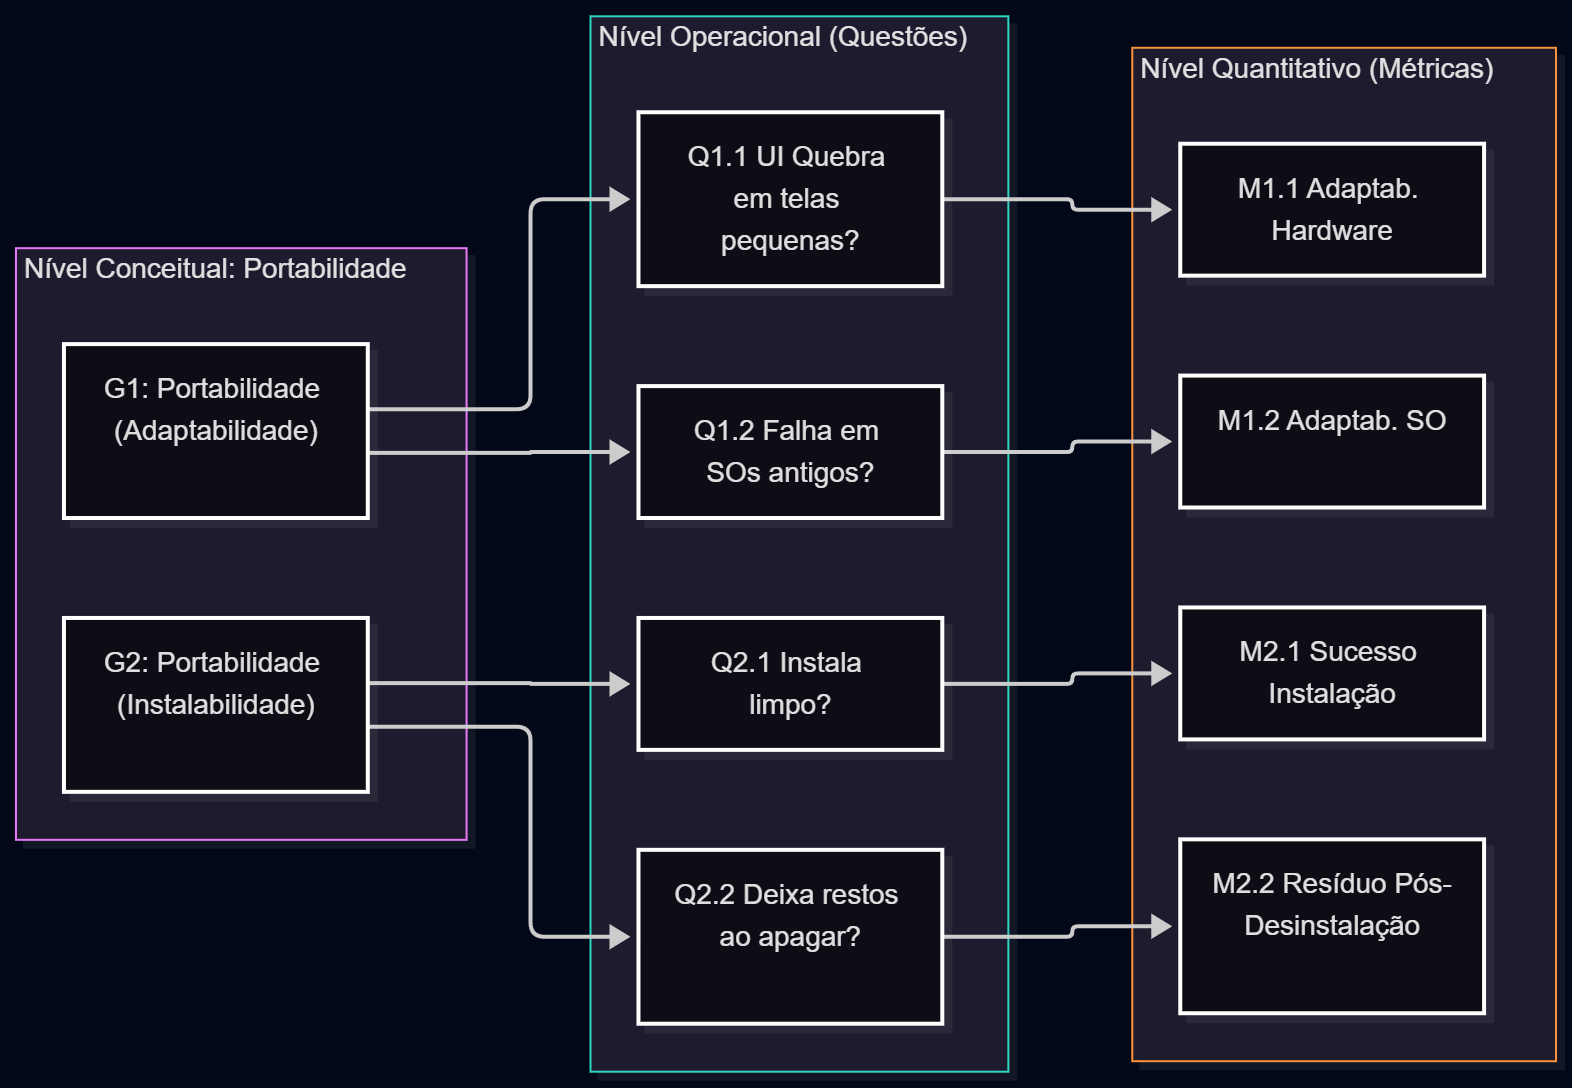
\includegraphics[width=0.7\textwidth]{images/mermaid-diagram-2026-10-31-162443.png}
\caption{Diagrama GQM focado em Portabilidade (Adaptabilidade e Instalabilidade).}
\label{fig:gqm_portabilidade}
\end{figure}

\begin{figure}[H]
\centering
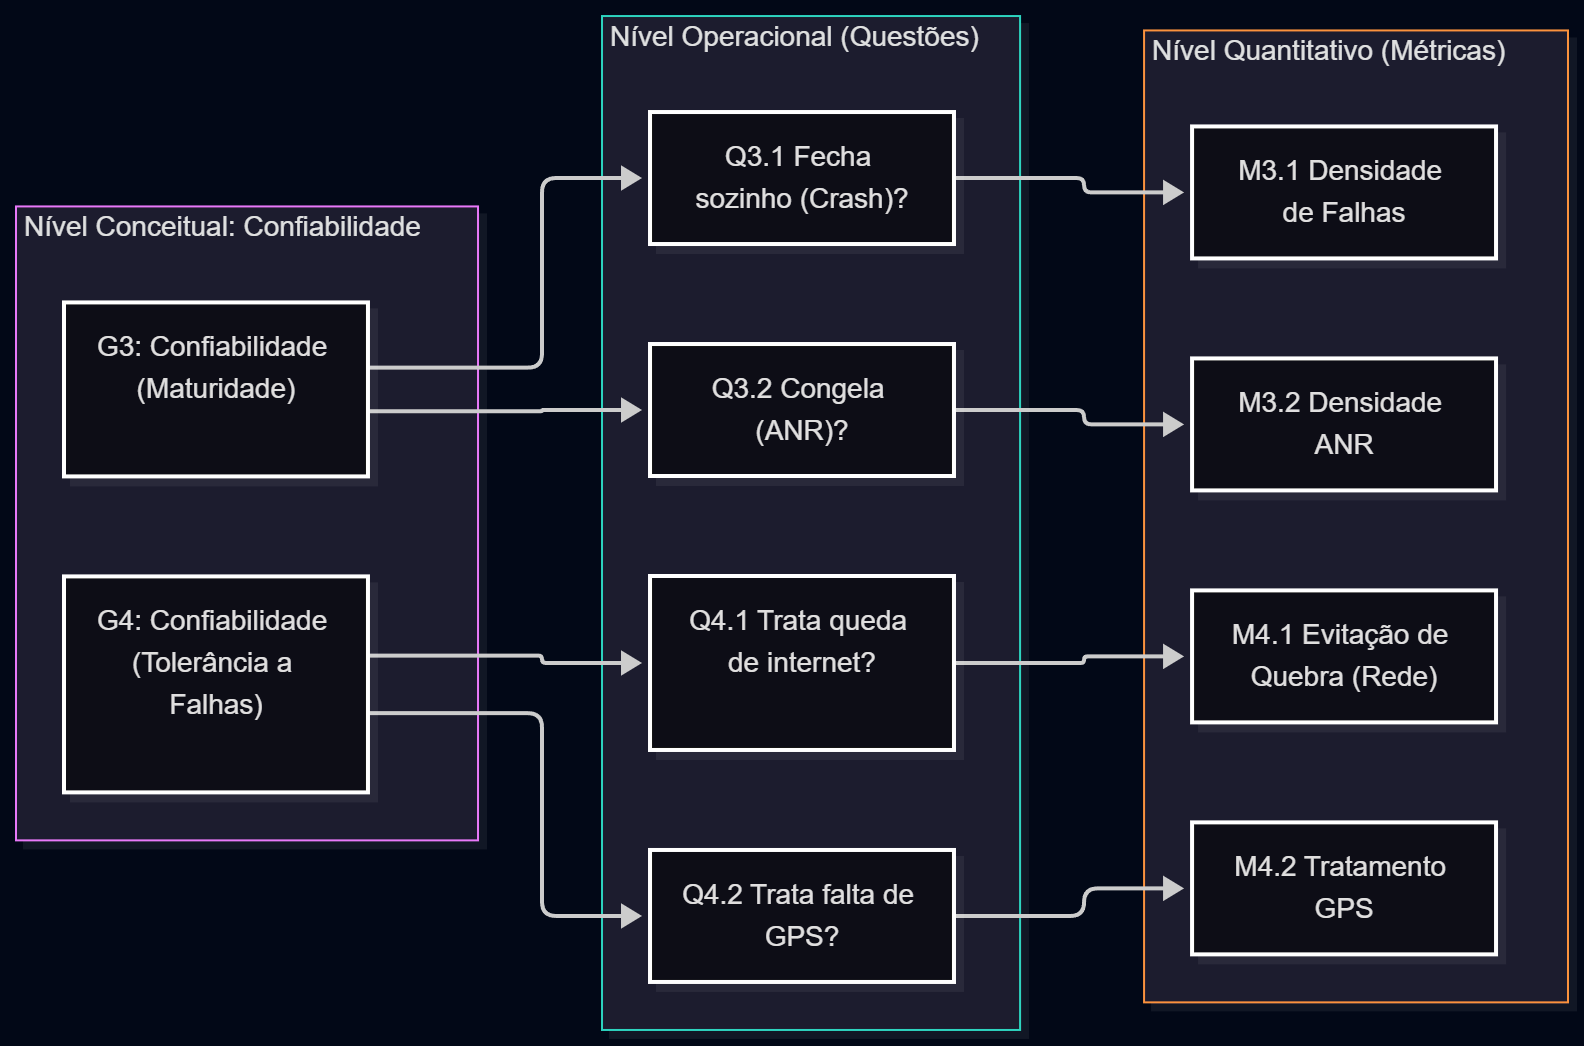
\includegraphics[width=0.7\textwidth]{images/mermaid-diagram-2026-10-31-162527.png}
\caption{Diagrama GQM focado em Confiabilidade (Maturidade e Tolerância a Falhas).}
\label{fig:gqm_confiabilidade}
\end{figure}

\begin{figure}[H]
\centering
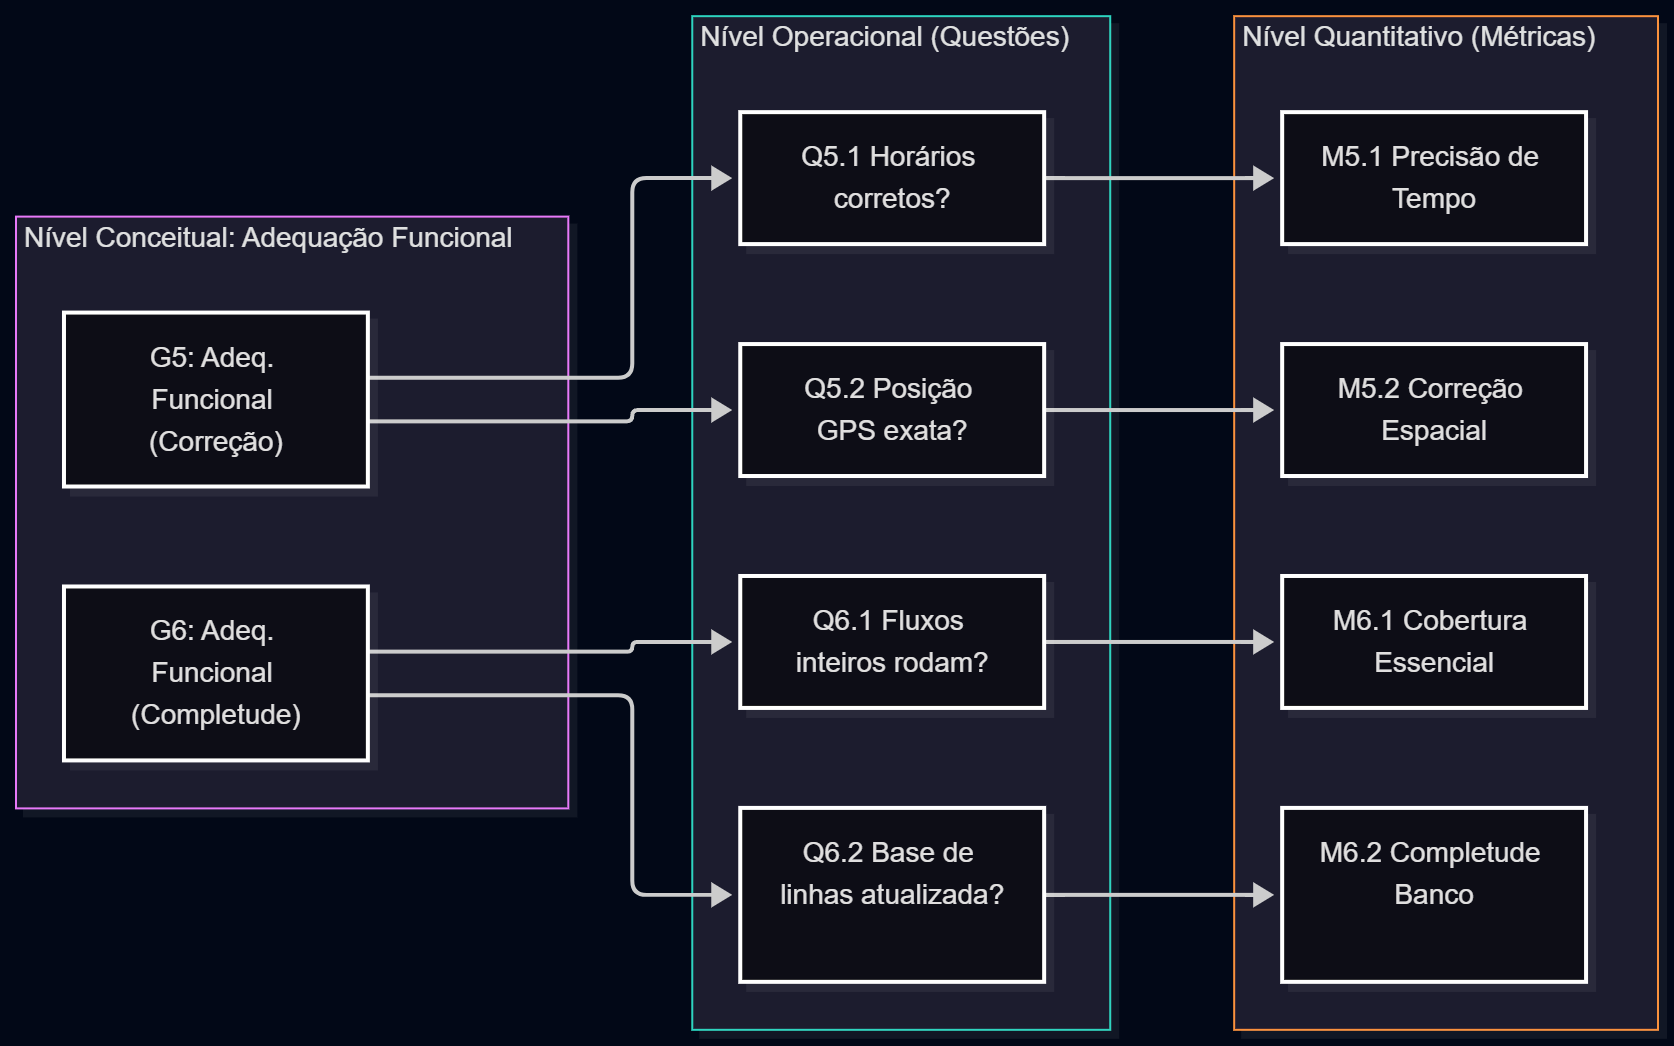
\includegraphics[width=0.7\textwidth]{images/mermaid-diagram-2026-10-31-162600.png}
\caption{Diagrama GQM focado em Adequação Funcional (Correção e Completude).}
\label{fig:gqm_adequacao}
\end{figure}

\subsection{Terminologia e Conceitos no Contexto do Projeto}
\label{sec:terminologia}

A terminologia empregada é restrita ao escopo do trabalho e adaptada ao
contexto do produto: os nomes das características e subcaracterísticas
seguem a ISO/IEC 25010~\cite{iso25010} (maturidade, tolerância a falhas,
adaptabilidade, completude, correção e pertinência funcionais), e os termos
de medição seguem o GQM~\cite{basili1988,basili1994}. Conceitos externos ao escopo da
avaliação foram deliberadamente omitidos para evitar jargão irrelevante, e o
texto foi unificado no português do Brasil.

\subsection{Declaração de Uso de Inteligência Artificial}
\label{sec:ia}

Em atendimento aos critérios de avaliação da disciplina, declaramos que
utilizamos modelos de Inteligência Artificial (Gemini e ChatGPT) para
auxiliar nas tarefas de formatação de tabelas, adequação do código para
\LaTeX, estruturação das subcaracterísticas GQM e revisão gramatical e
ortográfica do texto. Todo o conteúdo gerado foi integralmente lido,
validado, ajustado tecnicamente e consolidado pela equipe, incluindo a
unificação da terminologia em português do Brasil e a conferência dos
conceitos contra a norma ISO/IEC 25010, para garantir a coerência total com o
escopo do projeto e o rigor da disciplina. Não há inclusão bruta de respostas
das ferramentas, ícones de aplicativos ou alucinações não mitigadas neste
documento.

% ---------------------------------------------------------------------
\begin{thebibliography}{99}

\bibitem{basili1988}
BASILI, V. R.; ROMBACH, H. D. The TAME Project: Towards Improvement-Oriented
Software Environments. \emph{IEEE Transactions on Software Engineering},
v.~14, n.~6, p.~758--773, jun. 1988.

\bibitem{basili1994}
BASILI, V. R.; CALDIERA, G.; ROMBACH, H. D. The Goal Question Metric
Approach. In: MARCINIAK, J. J. (ed.). \emph{Encyclopedia of Software
Engineering}. New York: John Wiley \& Sons, 1994. v. 1, p. 528--532.

\bibitem{deissenboeck2009}
DEISSENBOECK, F.; JUERGENS, E.; LOCHMANN, K.; WAGNER, S. Software Quality
Models: Purposes, Usage Scenarios and Requirements. In: \emph{Proceedings of
the 7th International Workshop on Software Quality (WoSQ)}. Los Alamitos:
IEEE, 2009. p.~9--14.

\bibitem{khalid2015}
KHALID, H.; SHIHAB, E.; NAGAPPAN, M.; HASSAN, A. E. What Do Mobile App
Users Complain About? \emph{IEEE Software}, v.~32, n.~3, p.~70--77,
mai./jun. 2015.

\bibitem{minelli2015}
MINELLI, R.; MOCCI, A.; LANZA, M. I Know What You Did Last Summer: An
Investigation of How Developers Spend Their Time. In: \emph{Proceedings of
the 23rd IEEE International Conference on Program Comprehension (ICPC)}.
Los Alamitos: IEEE, 2015. p.~25--35.

\bibitem{iso25000}
ISO/IEC. \emph{ISO/IEC 25000:2014} --- Systems and software Quality
Requirements and Evaluation (SQuaRE): Guide to SQuaRE. Genebra: ISO/IEC,
2014.

\bibitem{iso25010}
ISO/IEC. \emph{ISO/IEC 25010:2011} --- Systems and software Quality
Requirements and Evaluation (SQuaRE): System and software quality models.
Genebra: ISO/IEC, 2011.

\bibitem{iso25040}
ISO/IEC. \emph{ISO/IEC 25040:2011} --- Systems and software Quality
Requirements and Evaluation (SQuaRE): Evaluation process. Genebra: ISO/IEC,
2011.

\bibitem{onu2015}
ORGANIZAÇÃO DAS NAÇÕES UNIDAS (ONU). \emph{Transformando nosso mundo: a
Agenda 2030 para o Desenvolvimento Sustentável}. Nova York: ONU, 2015.

\bibitem{fcte2026}
FCTE --- QUALIDADE DE SOFTWARE 1. \emph{2026-2\_T02\_CAROL\_SHAW: repositório
do projeto e GitPage da equipe}. Disponível em:
\url{https://github.com/FCTE-Qualidade-de-Software-1/2026-2_T02_CAROL_SHAW}.
Acesso em: 20 out. 2026.

\bibitem{semob2026}
GOVERNO DO DISTRITO FEDERAL. \emph{Semob-DF: aplicativo DF no Ponto}.
Disponível em: \url{https://www.semob.df.gov.br/}. Acesso em: 20 out. 2026.

\end{thebibliography}

% ---------------------------------------------------------------------
\appendix
\section{Tabela de Contribuição da Equipe}
\label{ap:contribuicao}

A Tabela~\ref{tab:contribuicao} detalha a divisão de trabalho e o esforço de
cada membro nesta primeira entrega, conforme exigido pelas premissas do
projeto.

\begin{table}[h]
\centering
\caption{Contribuição e esforço dos membros da equipe na Entrega 1.}
\label{tab:contribuicao}
\footnotesize
\renewcommand{\arraystretch}{0.9}
\begin{tabularx}{\textwidth}{>{\raggedright\arraybackslash}p{4.3cm} X c}
\toprule
\textbf{Membro da equipe} & \textbf{Responsabilidades / tarefas realizadas} &
\textbf{Esforço} \\
\midrule
Cristiano Borges de Morais & Estruturação do referencial teórico e do modelo
ISO 25010 (Fase 1) & 16,6\% \\
João Guilherme Capozzi Gonçalves & Mapeamento do escopo e elaboração das
justificativas técnicas & 16,6\% \\
João Guilherme Lima Veras Fonseca & Formulação das métricas quantitativas
GQM (Fase 2) & 16,7\% \\
Pedro Ramos Sousa Reis & Organização do relatório em \LaTeX\ e do GitPage &
16,7\% \\
Rodrigo Braz Ferreira Gontijo & Definição dos objetivos, questões e hipóteses
GQM (Fase 2) & 16,7\% \\
Vitor Pereira Bessa & Análise de requisitos, metodologia e revisão técnica
global & 16,7\% \\
\midrule
\textbf{Total} & & \textbf{100\%} \\
\bottomrule
\end{tabularx}
\end{table}

\end{document}
